\chapter{Bateria}

\section*{Informações de segurança}

Leia toda a informação de segurança descrita nesta seção antes de instalar e de operar o equipamento. Não negligencie nenhuma instrução.

Para manipular e operar os sistemas de baterias:

\begin{itemize}

    \item Você deve ter qualificação para trabalhos com eletricidade;
    \item Remover todo e qualquer adereço metálico como joias, relógios, pulseiras, canetas e
barras metálicas antes de começar a manusear a bateria;
    \item Usar somente ferramentas eletricamente isoladas.

\end{itemize}

\subsection*{Simbologia de segurança e recomendações}


\begin{center}
    \begin{figure}[H]
    \centering
		
\includegraphics[scale=1.6]{Figuras/bateria/iconeimportante.png}
	    \label{iconeimportante}
    \end{figure} 
  
    	Informação importante sobre \textbf{SEGURANÇA}
 \end{center}   	
 
 \begin{center}
  
    \begin{figure}[H]
       \centering
	\label{iconefogo}					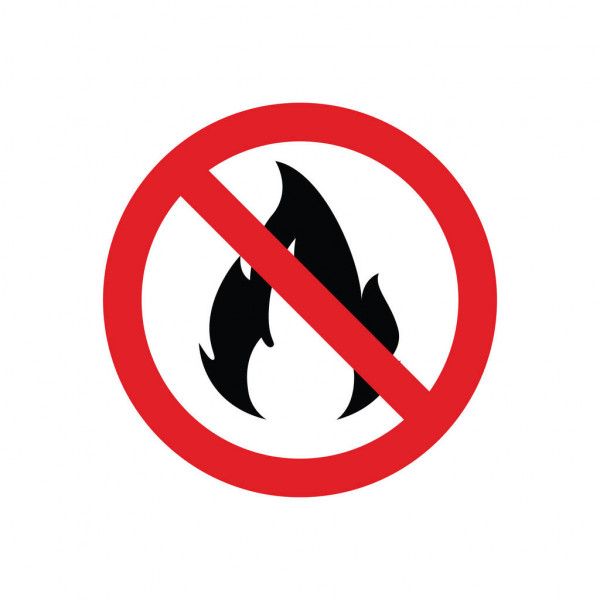
\includegraphics[keepaspectratio=true,scale=0.13]{Figuras/bateria/iconefogo.jpg}
        \label{iconefogo}
	\end{figure} 
		\textbf{NÃO} atirar a bateria ao fogo
\end{center}

\begin{center}
    \begin{figure}[H]
\centering
	\label{iconereciclar}					
\includegraphics[keepaspectratio=true,scale=0.13]{Figuras/bateria/iconereciclar.png}
        \label{iconereciclar}
	
	\end{figure} 
	\textbf{RECICLAR} ou descartar corretamente à bateria
 \end{center}   
 
 \begin{center}

  \begin{figure}[H]
  \centering
	\label{iconelixo}					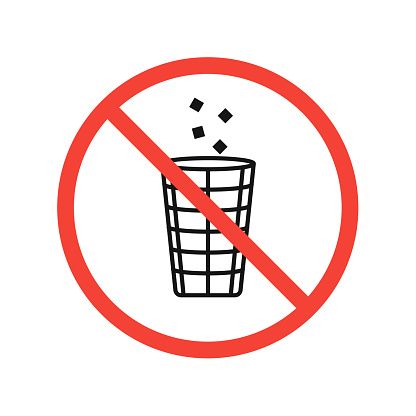
\includegraphics[keepaspectratio=true,scale=0.7]{Figuras/bateria/iconelixo.jpg}
        \label{iconelixo}
	
	\end{figure} 
      \textbf{NÃO} descartar a bateria em lixo comum.
 \end{center}  
\subsection*{Cuidados}
    
    \begin{figure}[H]
    \centering
	\label{iconeimportante}
		
\includegraphics[keepaspectratio=true,scale=1.4]{Figuras/bateria/iconeimportante.png}
	\label{iconeimportante}
	\end{figure} 
    
    \begin{enumerate}
    \item \textbf{NÃO} colocar a bateria na água. Armazenar a bateria em local fresco e seco, sem incidência direta do sol.
	\item \textbf{NÃO }aquecer ou jogar a bateria no fogo. Risco de explosão e/ou incêndio. 
\item Quando recarregar a bateria, utilizar equipamento especialmente projetado para isso e seguir os corretos procedimentos e parâmetros de uso. \textbf{NÃO }utilizar carregadores inadequados ou fora da especificação. \textbf{NÃO} realizar adaptações.
\item  \textbf{NÃO} reverter a polaridade da bateria. \textbf{NÃO} conectar a bateria diretamente na rede AC e evitar o curto-circuito entre os terminais.
\item  \textbf{NÃO} utilizar a bateria caso ela se torne quente, abaulada, deformada ou que apresente vazamentos.
\item \textbf{NÃO} perfurar a bateria. \textbf{NÃO } jogar, amassar ou causar impacto físico à bateria.
\item \textbf{NÃO} abrir ou tentar reparar a bateria em caso de defeito pois, além de perigoso, a garantia é invalidada caso ela tenha sido aberta para reparo por pessoal não autorizado pelo fornecedor.
\item \textbf{NÃO} descartar a bateria no lixo comum, procurar pontos de recolhimento para a correta destinação ou reciclagem.
    \end{enumerate}

    \subsection*{Precauções}
\begin{figure}[H]
\centering
	\label{iconeimportante}
		
\includegraphics[keepaspectratio=true,scale=1.6]{Figuras/bateria/iconeimportante.png}
	\label{iconeimportante}
	\end{figure} 
    
\begin{enumerate}
\item Caso a bateria esteja aquecida, abaulada, com odor ou aspecto anormal, entrar imediatamente em contato com o suporte e não usar a bateria.
\item  Caso precise armazenar a bateria por longos períodos, realizar uma carga e descarga com a bateria a cada 3 meses. Para assegurar o melhor desempenho e o melhor estado de carga, manter a bateria armazenada com carga entre 50\% e 60\%.
\item Utilizar a bateria apenas na faixa de temperatura adequada, entre -20ºC e 60ºC.
\item Antes da primeira utilização é recomendado recarregar a bateria.
\end{enumerate}
\newpage   

\section*{Troca das baterias}
\begin{figure}[H]
\centering
	\label{iconeimportante}
		
\includegraphics[keepaspectratio=true,scale=1.7]{Figuras/bateria/iconeimportante.png}
		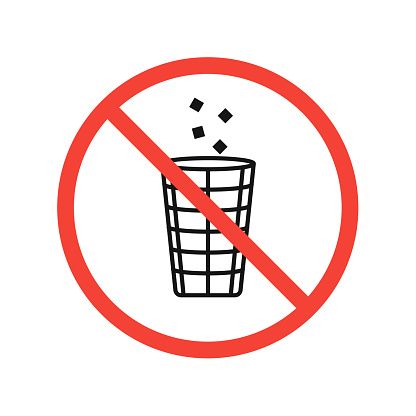
\includegraphics[keepaspectratio=true,scale=0.5]{Figuras/bateria/iconelixo.jpg}
	\label{iconeimportante}
	\end{figure} 
As baterias têm vida útil variável, e após determinado número de ciclos, de carga e descarga, perdem a capacidade de carga e devem ser substituídas.

Estima-se que o número de ciclos antes que ocorra essa perca na capacidade de carga seja superior a 4000. Porém, esse número pode variar de acordo com as condições de operação, armazenamento e recarga das baterias. 

Portanto, deve-se observar a situação de capacidade de carga das baterias periodicamente para se atentar a necessidade de trocas. A cada três meses recomenda-se ligar o sistema completo para testar por quanto tempo as baterias são capazes de manter todos os componentes alimentados. Dessa forma é possível observar a redução da capacidade das baterias com o passar do tempo e realizar a troca quando essa capacidade estiver muito próxima do necessário para os lançamentos remotos.

Para realizar a troca garanta que o dispositivo esteja desconectado da rede elétrica, então obedecendo todas as normas de segurança já estabelecidas nesse manual, retire a estrutura que protege a bateria usando chave de fenda, após isso desconecte todos os fios que estão presos a bateria com muito cuidado, no caso da bateria da maleta apenas desconecte o conector dock acoplado ao polos da bateria, depois troque pela nova bateria que deve ser do mesmo tipo (tamanho, tensão e capacidade) que a antiga. 

Depois de colocar a bateria nova no lugar repita as conexões que estavam na bateria anterior com cuidado e observando onde é o polo positivo (conexões com os fios de cor vermelha) e o polo negativo (conexões com os fios de cor preta) da bateria, no caso da bateria da maleta apenas conecte novamente o conector dock nos polos. Depois de conectado volte a estrutura para o lugar e fixe com os parafusos.

\section*{Carregamento das baterias}

\subsection*{Tensão de alimentação do carregador}
  
Conferir a tensão de alimentação selecionada, 110V ou 220V, antes de cada uso. Selecionar a tensão de acordo com o rede elétrica do local de uso por meio da chave seletora de tensão, localizada na estrutura do carregador.

\subsection*{Carregando as baterias}

As baterias devem ser recarregadas após cada uso. 

Ao retornar com o sistema para um local com acesso à rede elétrica, conectar os cabos à caixa do carregador, selecionar a tensão de alimentação adequada no carregador e conectar os cabos à tomada e ao plugue P4 indicado para carregamento da bateria na estrutura do sistema. 

A conexão à rede deve ser contínua por 3 horas ininterruptas, após esse período mínimo a bateria estará carregada, não há problema em deixar a bateria conectada à rede por períodos mais longos, pois o circuito de carregamento faz o controle da tensão para manter a carga. 

Após carregar o primeiro sistema, maleta ou base de lançamento, repetir o procedimento para o segundo sistema.
